%include common packages and settings
\usepackage{etex} %эта магическая херь избавляет от переполнения регистров TeX а!!!

\mode<article>{\usepackage{fullpage}}
\mode<presentation>{
    \usetheme{Madrid} %%Boadilla,Madrid,AnnArbor,CambridgeUS,Malmoe,Singapore,Berlin
    \useoutertheme{shadow}
} 

\usepackage[utf8]{inputenc}
\usepackage[russian]{babel}
\usepackage{indentfirst}
\usepackage{graphicx}

\usepackage{amsmath}
\usepackage{amsfonts}
\usepackage{amsthm}

%\date{Место презентации \\(\today)}
\author[М.~М.~Шихов]{Михаил Шихов \\ \texttt{\underline{m.m.shihov@gmail.com}}}


\title[Полотно кастинговой сети]{Вяжем полотно кастинговой сети <<клиньями>>}

\begin{document}

\mode<article>{\maketitle\tableofcontents}
\frame<presentation>{\titlepage}
\begin{frame}<presentation>
    \frametitle{Содержание}
    \tableofcontents
\end{frame}

\begin{frame}
    \frametitle{Что делаем?}

	\begin{itemize}
		\item Разберемся в общих принципах вязания круглого сетевого полотна.
		\item Поймем через сколько обычных рядов нужно вязать ряд с добавками и сколько в этом ряду этих самых добавок должно быть. 
		\item Свяжем несколько маленьких полотен в качестве примера и посмотрим, что получается.
		\item Выведем основные формулы.
	\end{itemize}
\end{frame}


\section{Как вязать круглое сетевое полотно?}

\begin{frame}
    \frametitle{Ячейка сети --- штука подвижная}
    \framesubtitle{Вытягиваясь по ширине, она уменьшается по высоте (и наоборот)}

    \begin{center}
        \includegraphics[width=0.95\textwidth]{figs/cells-simple}
    \end{center}
\end{frame}


\subsection{Вяжем одним циллиндром без добавок}

\begin{frame}
    \frametitle{Если связать всё полотно одинм циллиндром}
    \framesubtitle{При этом верхнюю часть просто <<стянуть>> к горловине}

    \begin{center}
        \includegraphics[width=0.95\textwidth]{figs/by-one-cylinder}
    \end{center}
\end{frame}

\begin{frame}
    \frametitle{В <<стянутом>> циллиндре}
    \framesubtitle{Ячейки по краям полотна будут раскрыты, а у центра --- практически закрыты}

    \begin{center}
        \includegraphics[width=0.5\textwidth]{figs/cells-in-cylinder-mesh}
    \end{center}
\end{frame}

\begin{frame}
    \frametitle{Достоинства и недостатки}
	
	Достоинства:
    \begin{itemize}
        \item Не надо уметь вязать добавки.
    \end{itemize}
	
	Недостатки:
    \begin{itemize}
        \item Жуткая <<мотня>> из ячей в центре будет мешать забросу.
    \end{itemize}
	
	Надо подумать:
    \begin{itemize}
        \item Ячейки, <<закрытые>> в центре --- это достоинство или недостаток?
		\begin{itemize}
			\item Центр сети массивнее в полете.
			\item Центр сети оказывает большее сопротивление воде, когда сеть тонет (парашют лучше?).
		\end{itemize}		
    \end{itemize}
\end{frame}


\subsection{Вяжем <<Клиньями>>}

\begin{frame}
    \frametitle{Если взять циллиндр и вырезать лишнее,}
    \framesubtitle{то получатся клинья, в которых ячейки раскрыты равномерно}

    \begin{center}
        \includegraphics[width=0.99\textwidth]{figs/wedges}
    \end{center}
\end{frame}

\begin{frame}
    \frametitle{Сложив <<клинья>> на плоскость,}
    \framesubtitle{получим полотно с равномерным раскрытием ячеек}

    \begin{center}
        \includegraphics[width=0.43\textwidth]{figs/wedges-mesh-cells}
    \end{center}
\end{frame}

\begin{frame}
    \frametitle{Выводы}

	Когда полотно вяжется <<клиньями>>:
    \begin{itemize}
        \item Работы в два раза меньше, чем связать полотно одним циллиндром.
        \item Ячейки в полёте получаются равномерно раскрытыми.
		\item Клин легко формируется добавлеинем ячеи на ребре.
        \item Как будет видно, схема вязания клиньями по кругу очень простая и регулярная. Ошибиться тут сложно.
    \end{itemize}
\end{frame}


\subsection{Вяжем полотно из нескольких циллиндров}

\begin{frame}
    \frametitle{Вяжем несколькими циллиндрами}
    \framesubtitle{Чем меньше высота составляющих циллиндров, тем равномернее раскрытие ячей}

    \begin{center}
        \includegraphics[width=0.43\textwidth]{figs/by-many-cylinders}
    \end{center}
\end{frame}

\begin{frame}
    \frametitle{Полусфера несколькими циллиндрами}

    \begin{center}
        \includegraphics[width=0.35\textwidth]{figs/half-sphere}
    \end{center}
\end{frame}


\section{Как правильно делать добавки?}

\begin{frame}
    \frametitle{Как вязать добавку?}

%TODO    \begin{center}
%            \includegraphics[width=0.35\textwidth]{figs/addition-how-to}
%        \end{center}
\end{frame}


\subsection{Схемы вывязывания <<клина>>}

\begin{frame}
    \frametitle{Чтобы вязать <<клиньями>>}

    \begin{center}
        \includegraphics[width=0.7\textwidth]{figs/wedges}
    \end{center}

	надо определить:
    \begin{enumerate}
        \item Через сколько обычных рядов (провязаных циллиндром) нужно вязать ряд с добавками?
		\item Сколько в ряду c добавками этих самых добавок должно быть? Т.е. что то же: сколько <<клиньев>> надо вязать? 
    \end{enumerate}
\end{frame}

\begin{frame}
    \frametitle{Вяжем клин}
    \framesubtitle{Добавка каждый второй ряд. $M$=2}

    \begin{center}
        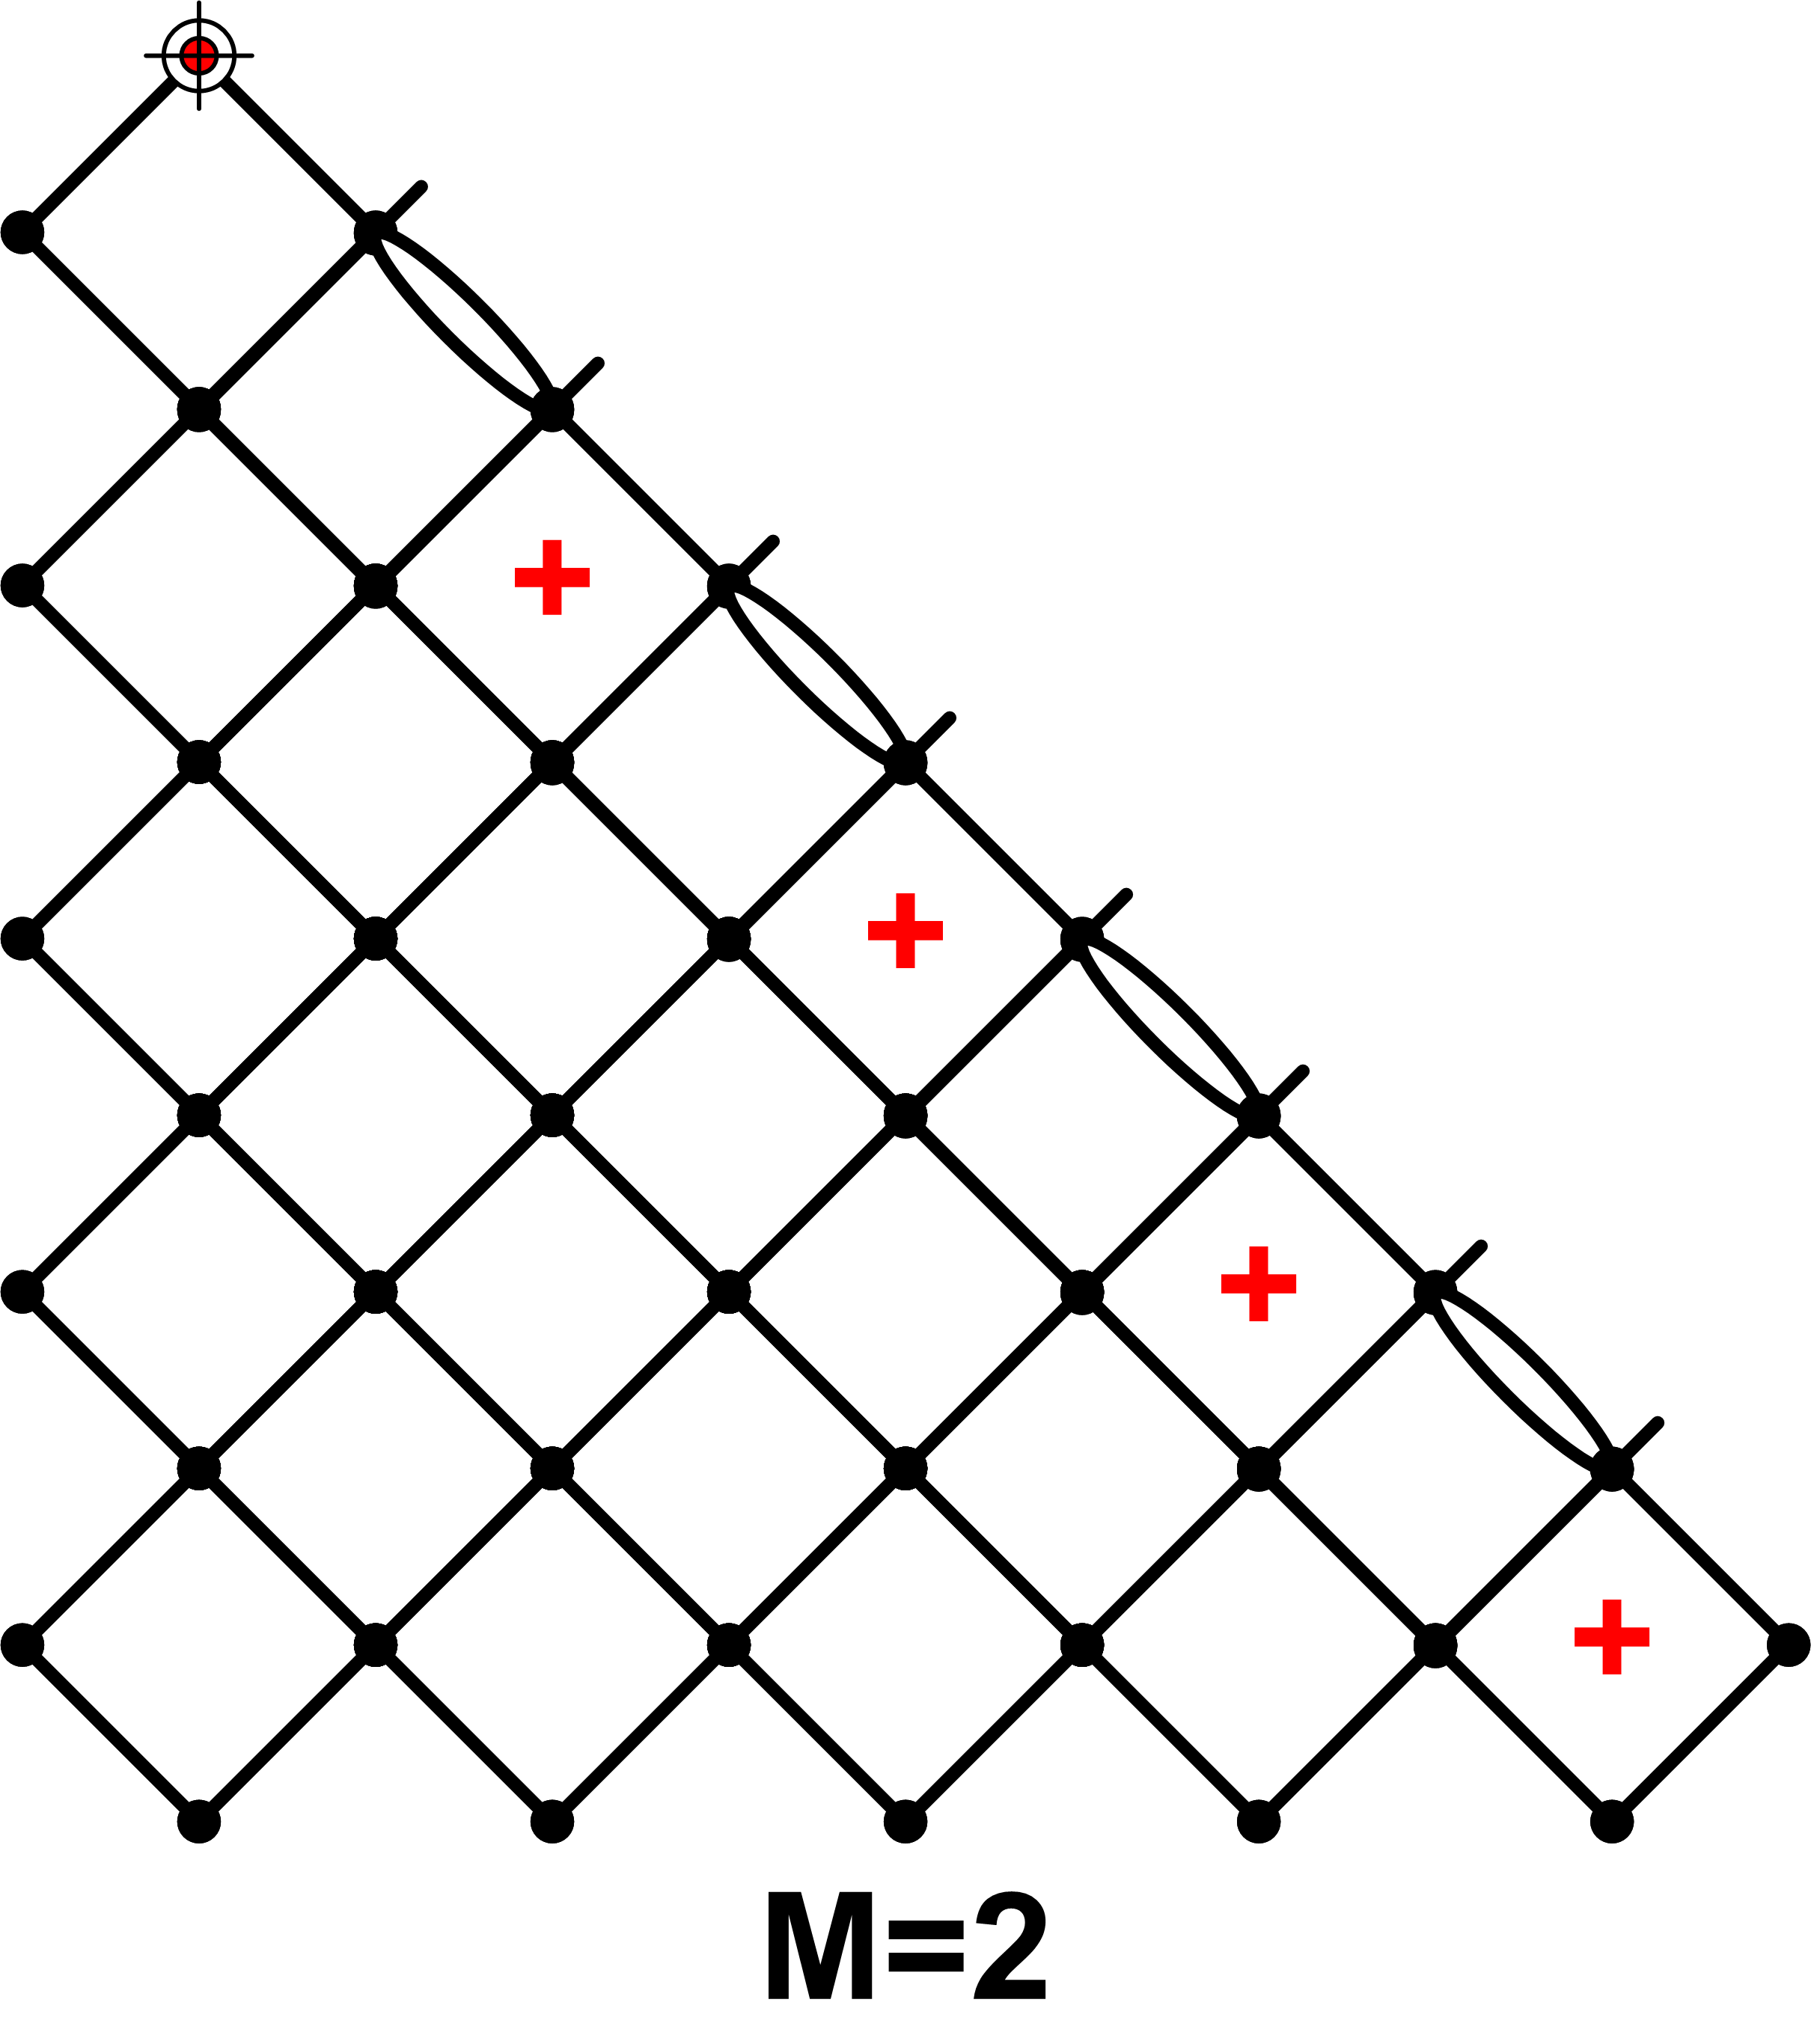
\includegraphics[width=0.5\textwidth]{figs/2b}
    \end{center}
\end{frame}

\begin{frame}
    \frametitle{Добавка каждый \alert{третий} ряд}

    \begin{center}
        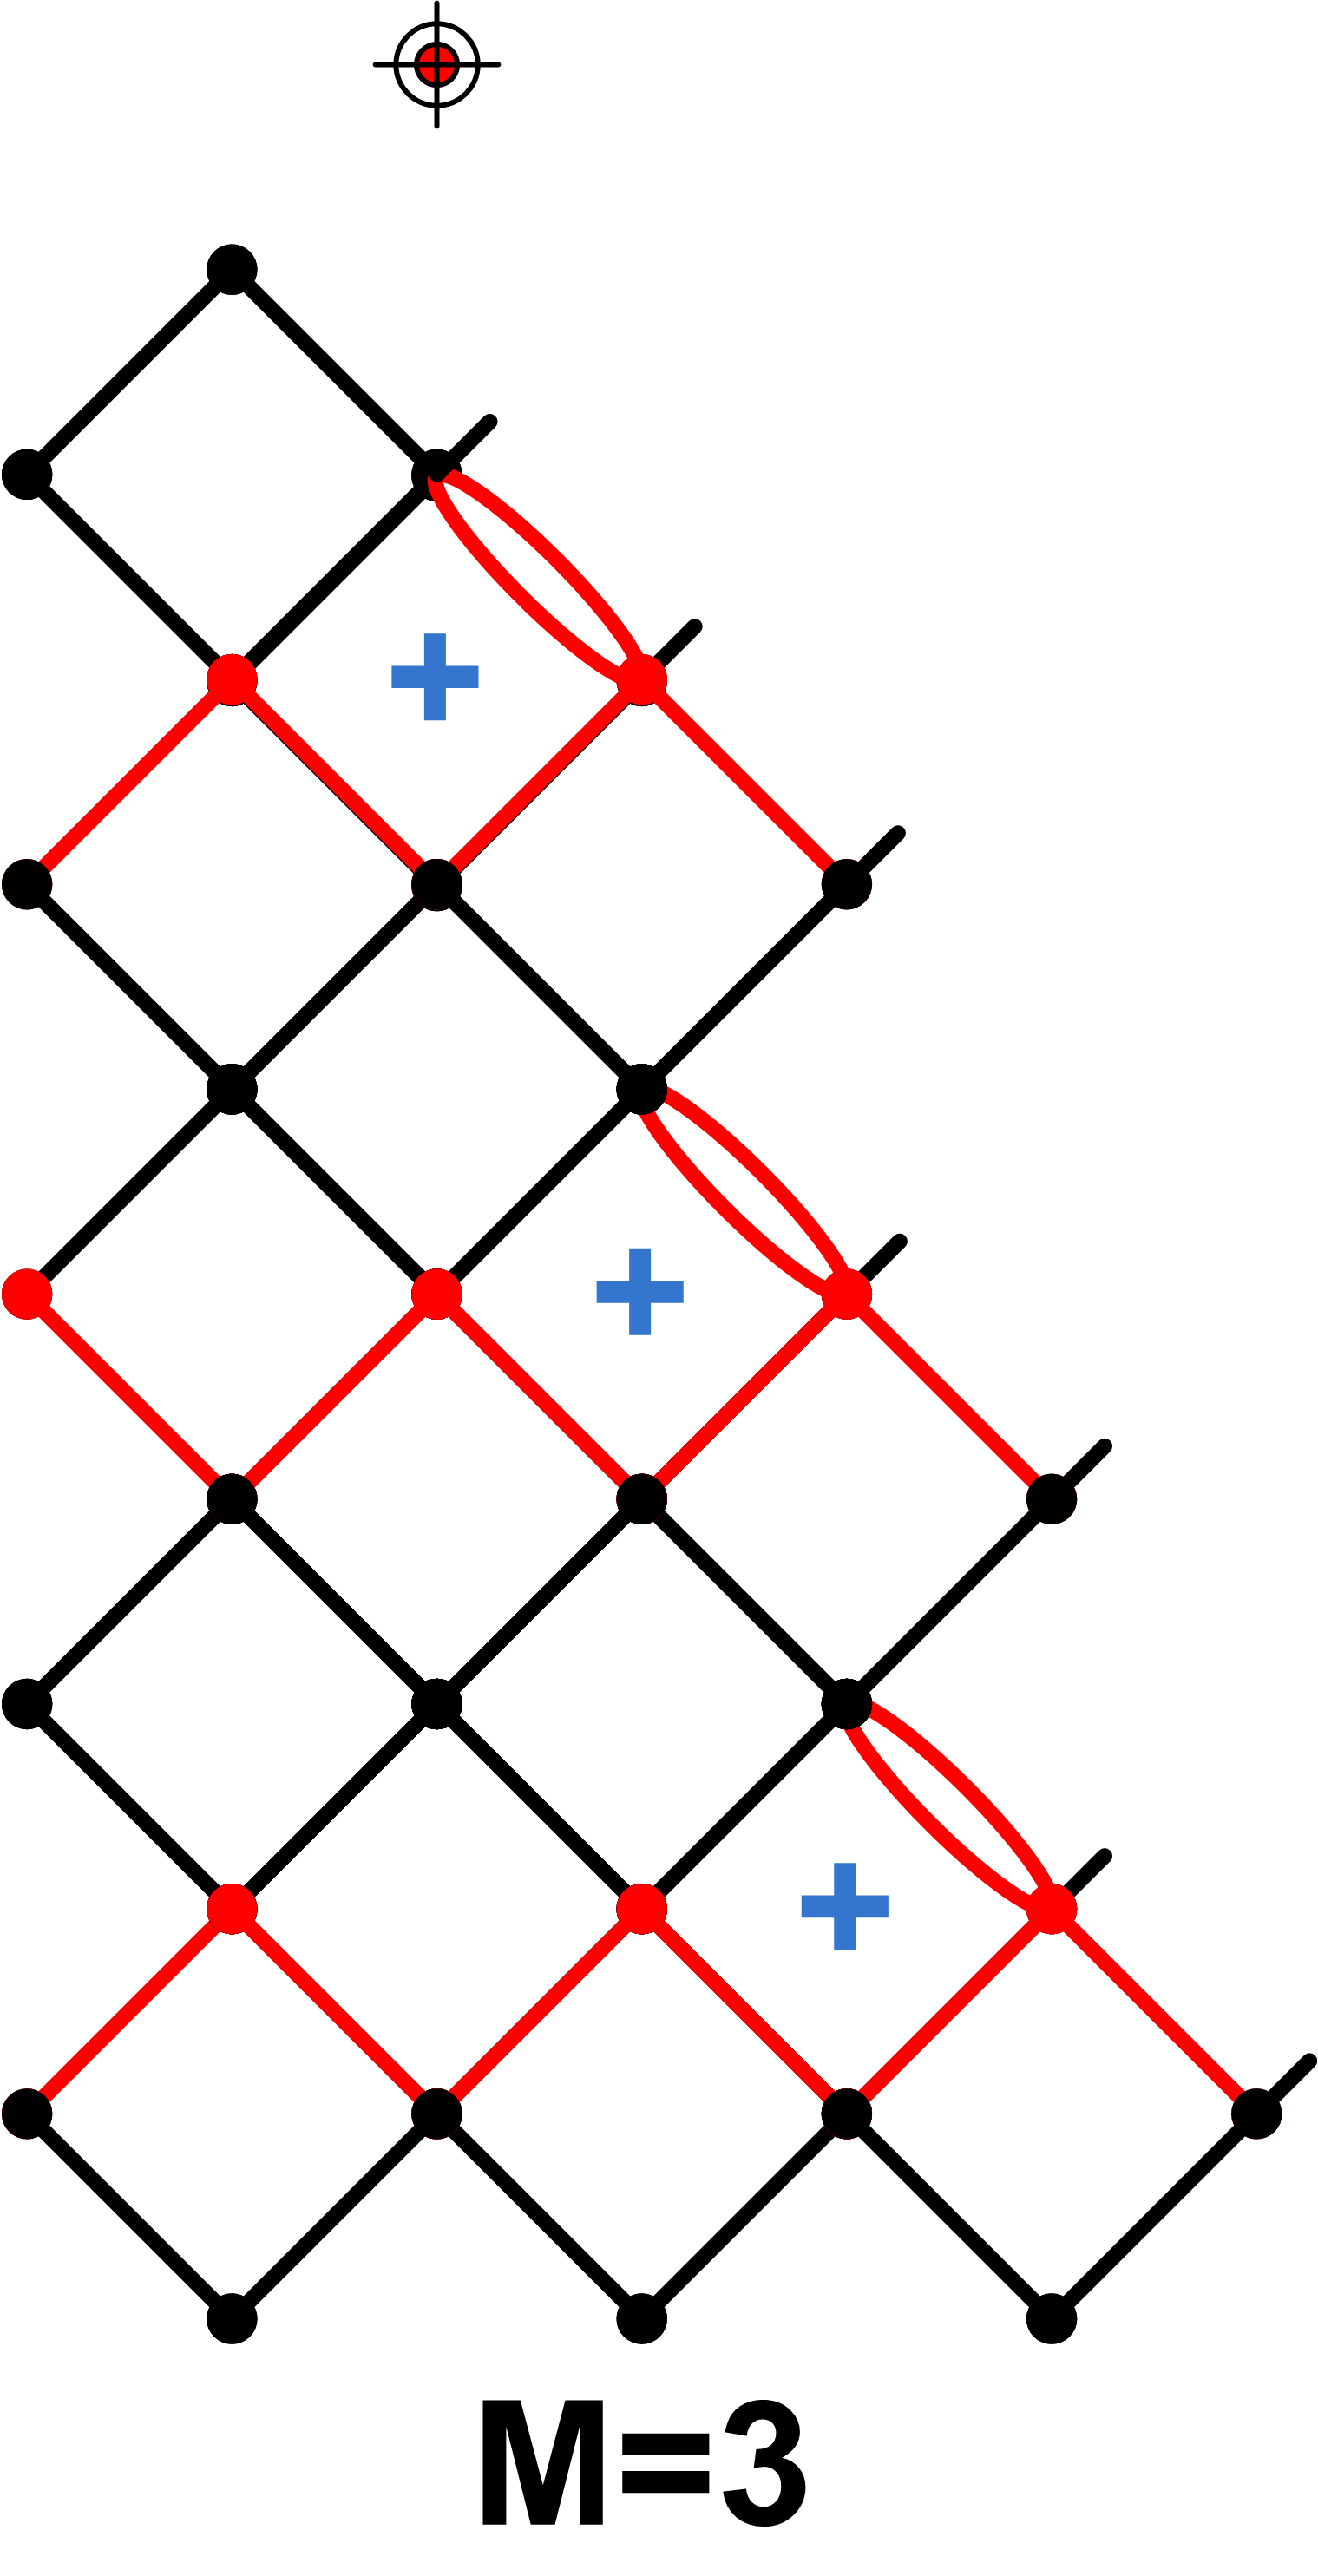
\includegraphics[width=0.3\textwidth]{figs/3b}
    \end{center}
\end{frame}

\begin{frame}
    \frametitle{Добавка каждый \alert{четвертый} ряд}

    \begin{center}
        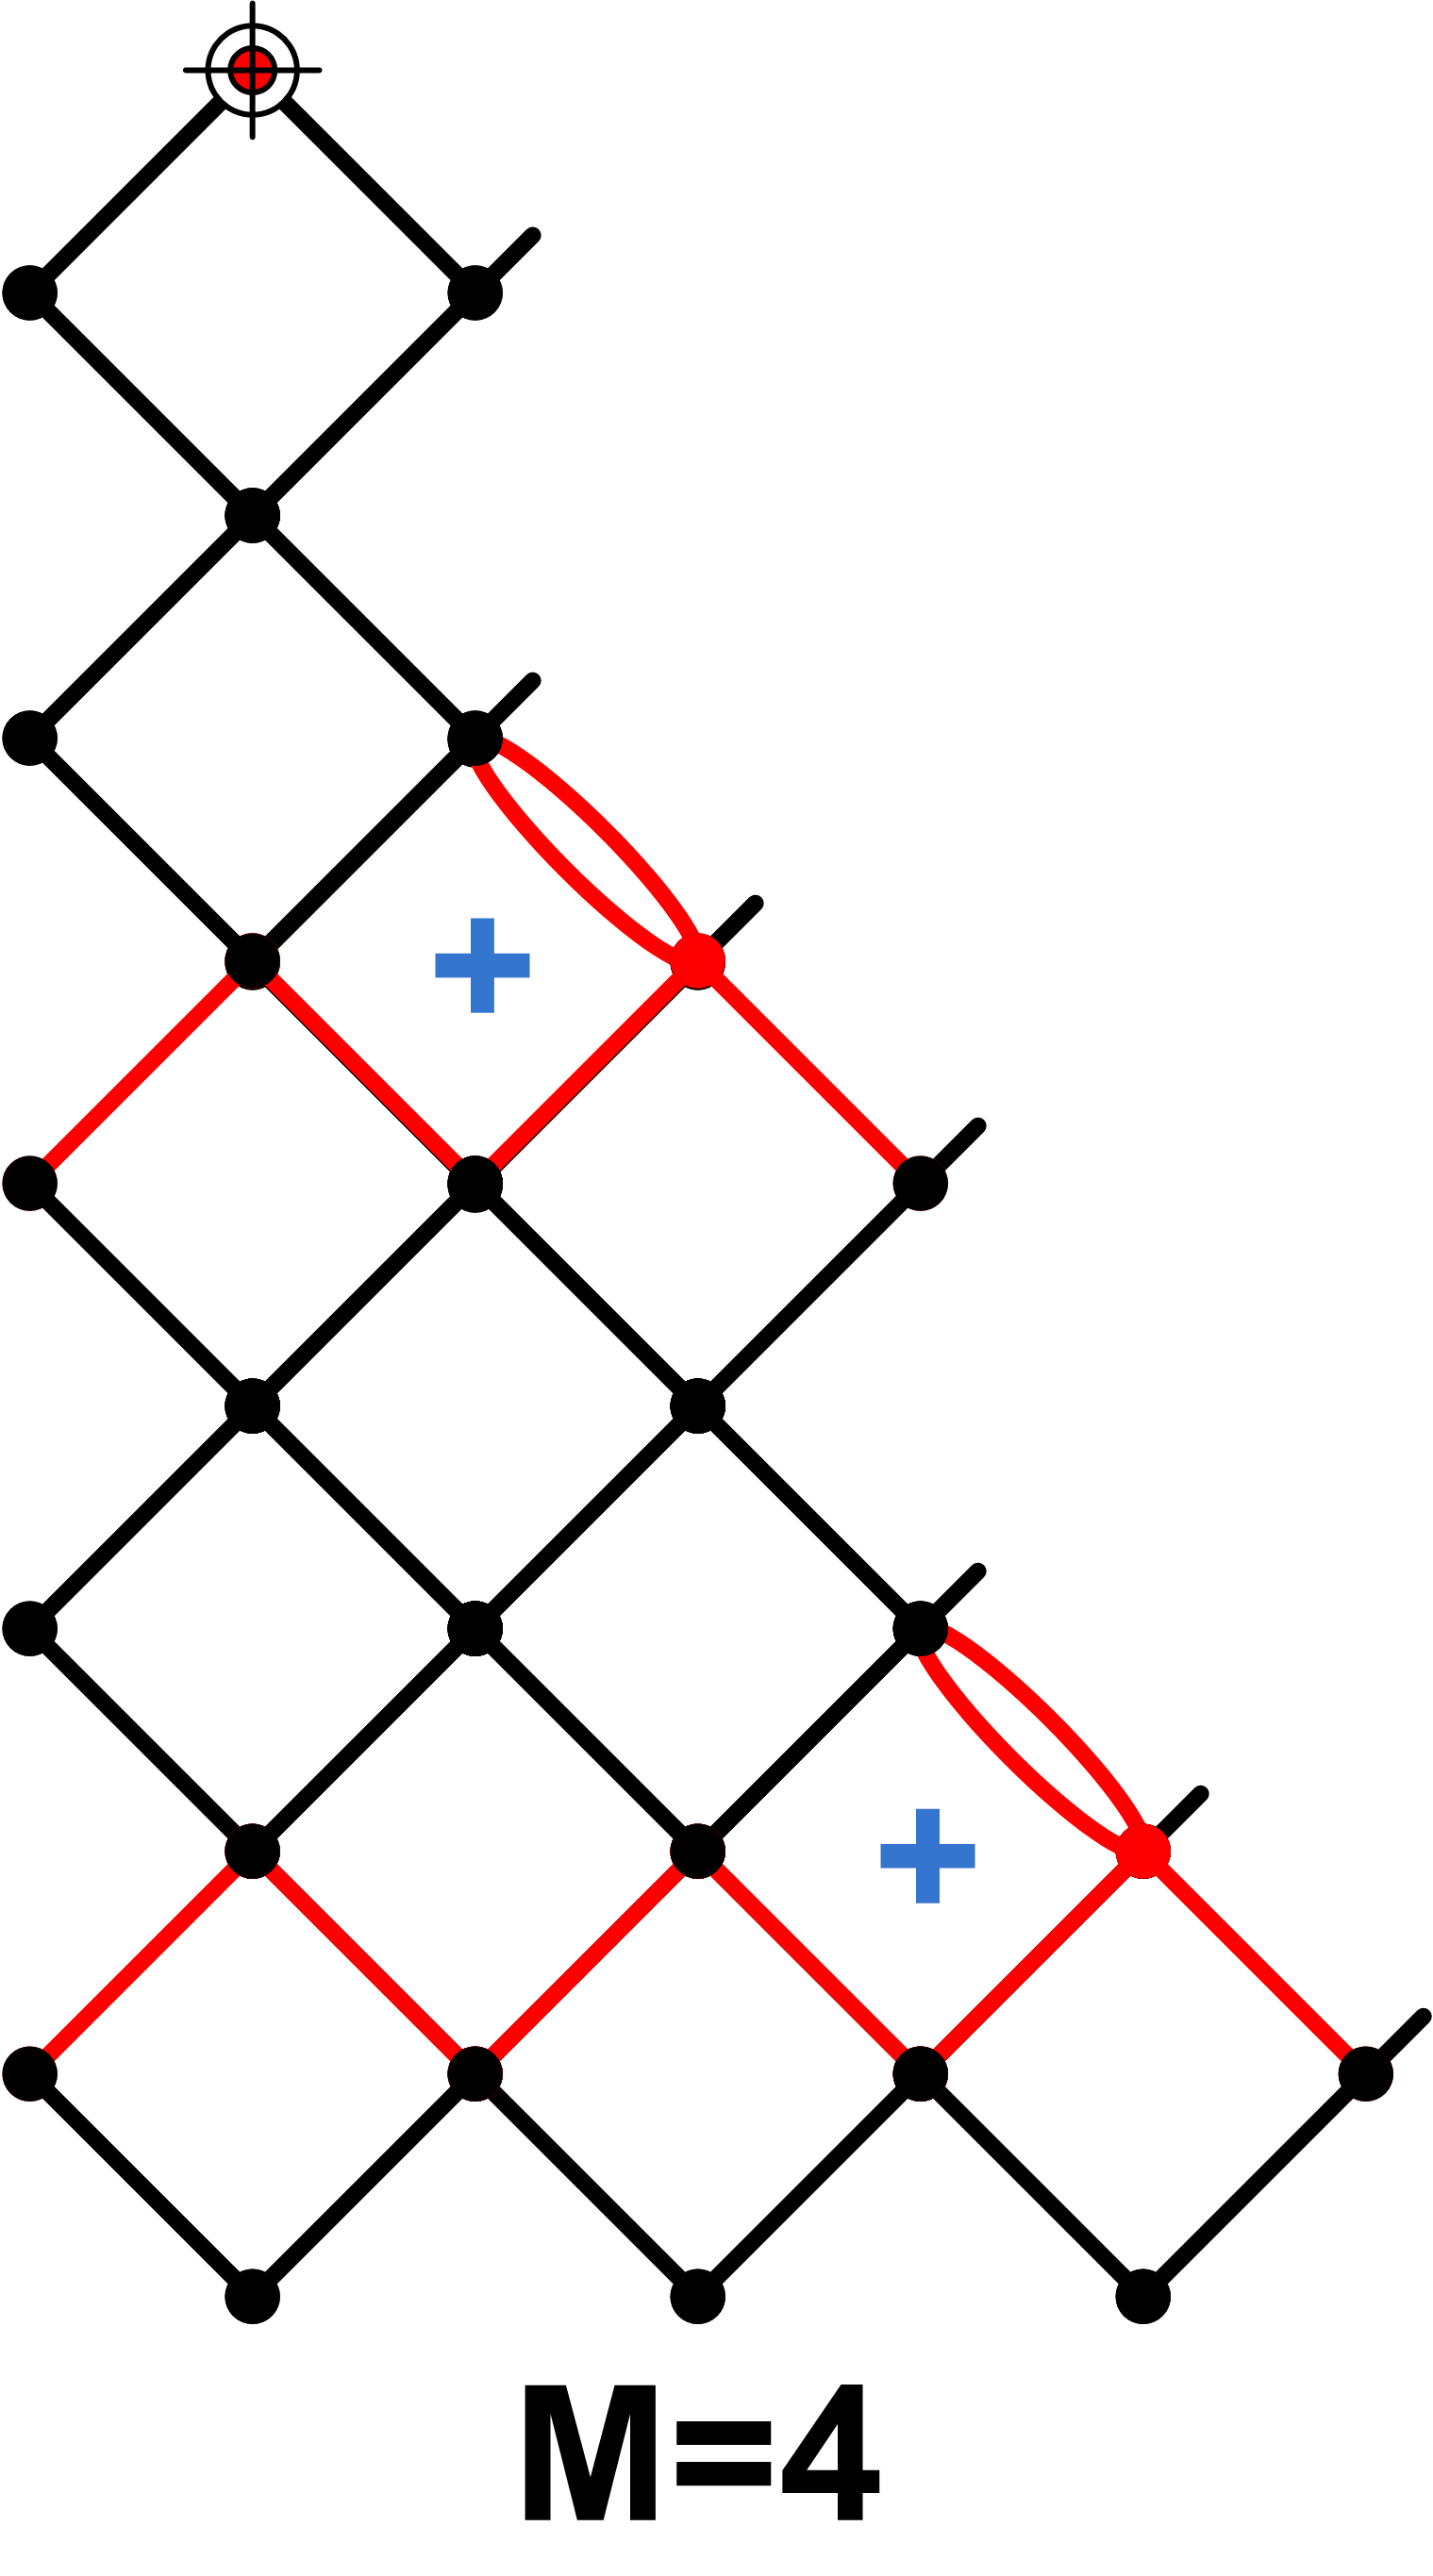
\includegraphics[width=0.3\textwidth]{figs/4b}
    \end{center}
\end{frame}

\begin{frame}
    \frametitle{Добавка каждый \alert{пятый} ряд}

    \begin{center}
        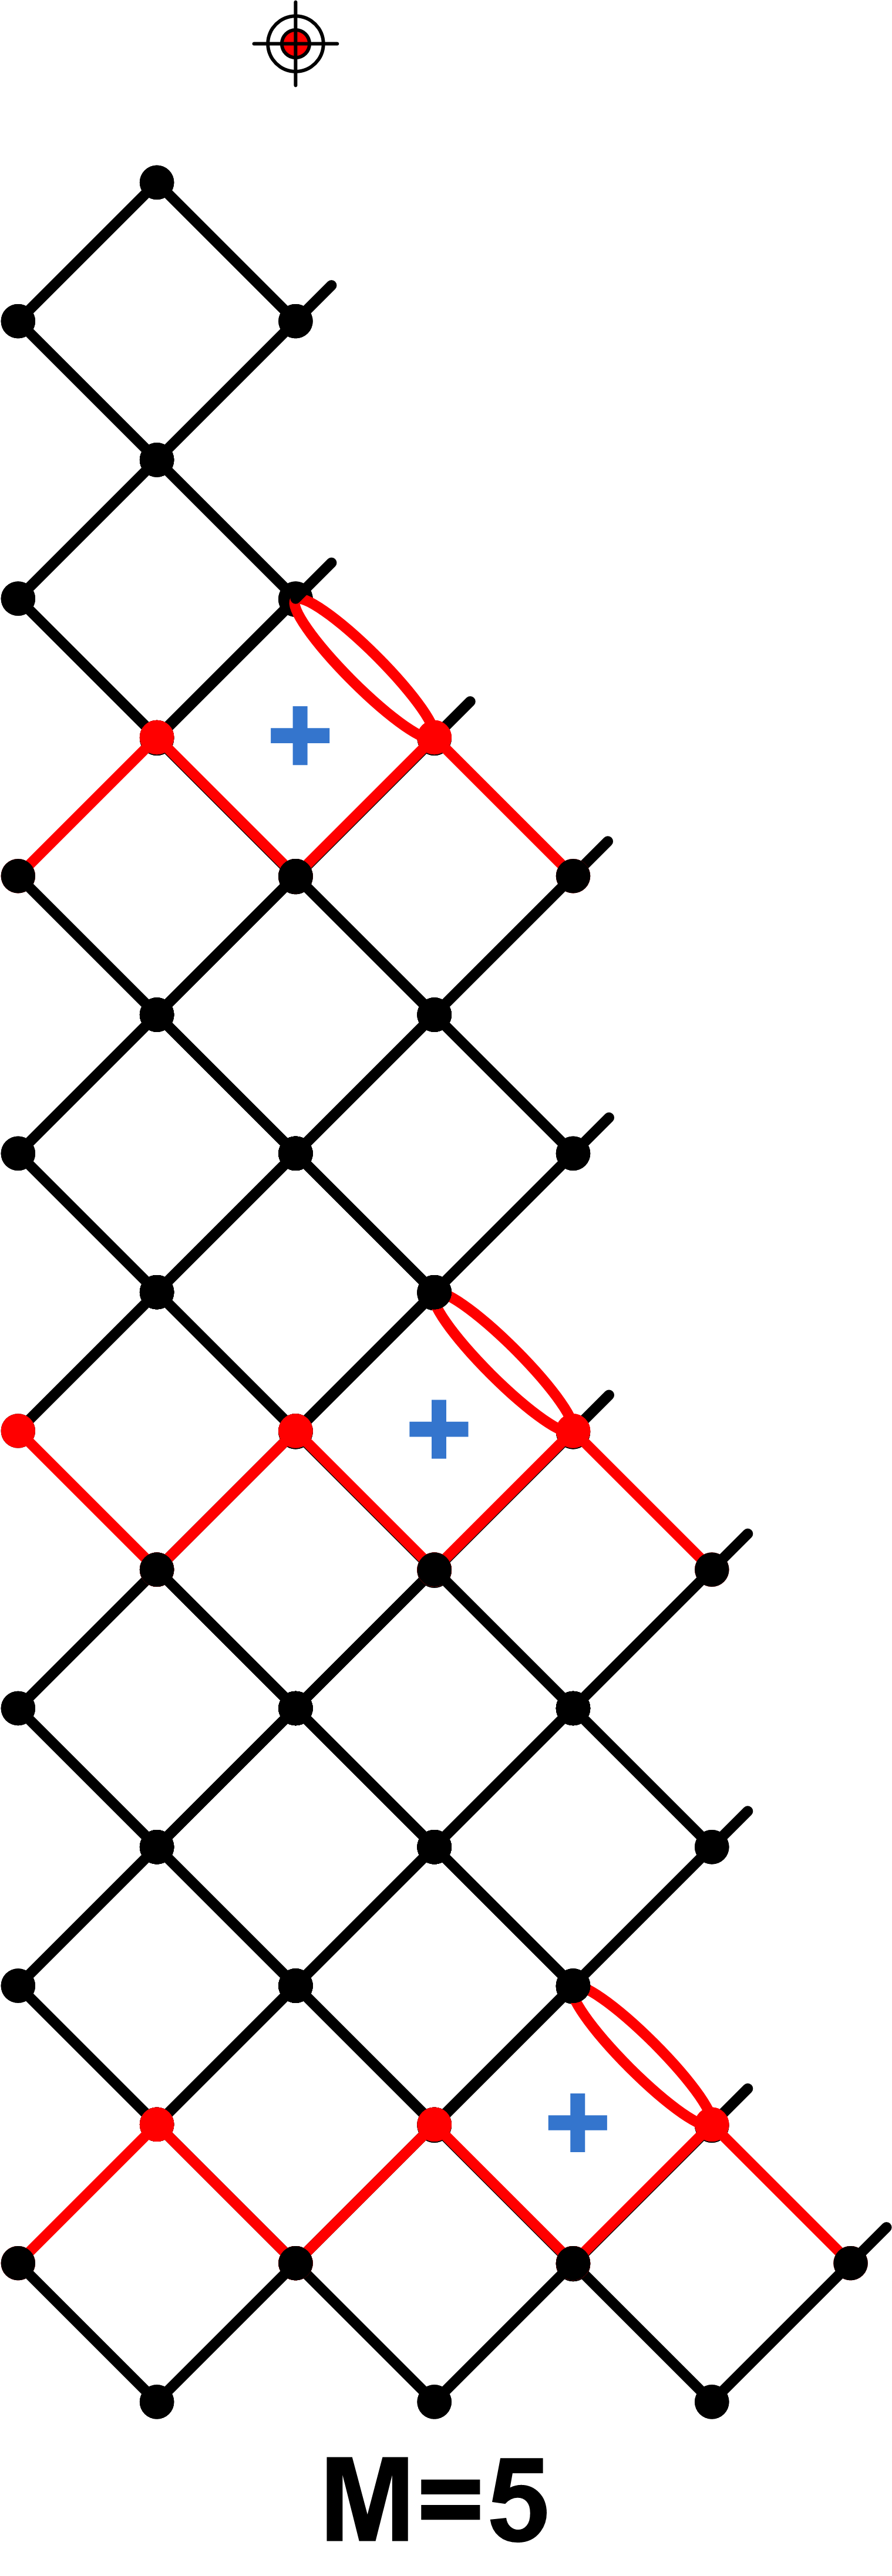
\includegraphics[width=0.2\textwidth]{figs/5b}
    \end{center}
\end{frame}


\subsection{Сколько добавок делать на ряд?}

\begin{frame}
    \frametitle{Обозначения для расчёта}

    \begin{center}
        \includegraphics[width=0.8\textwidth]{figs/round-proof}
    \end{center}
\end{frame}

\begin{frame}
    \frametitle{Обозначения для расчёта}

	\begin{itemize}
		\item $M$ --- добавки вяжем каждый $M$-й ряд (по одной из схем, см. рисунки выше); 
		\item $N$ --- количество добавок в <<добавочном>> ряду или, что то же, количество <<клиньев>>; 
		\item $c$ --- сторона ячейки в метрах (милиметрах);
		\item $a$ --- половинка высоты; 
		\item $b$ --- половинка ширины; 
		\item $r,R$ --- радиус раскрытой сети в метрах ($r$) и в рядах ($R$); 
		\item $s,S$ --- основание клина в метрах ($s$) и в ячеях ($S$).
	\end{itemize}
\end{frame}

\begin{frame}
    \frametitle{Насколько раскрыта ячейка?}
    \framesubtitle{Коэфициент <<полётного>> раскрытия: $k=\frac{a}{b}$}

    \begin{center}
        \includegraphics[width=0.9\textwidth]{figs/k}
    \end{center}
\end{frame}

\begin{frame}
    \frametitle{Как раскрытие ячейки $k$ зависит от $N$ и $M$}

	Радиус раскрытого полотна равен: $r=Ra$, а длина основания клина $s=2Sb$.
	
	Длина окружности может быть найдена как $Ns$ и как $2\pi r$. Следовательно:
	\begin{equation}
		\label{eq:circle-length}
		2NSb=2\pi Ra
	\end{equation}
	
	Так как добавка делается каждый $M$-й ряд, то количество ячеек в основании клина:
	\[
		S=\frac{R}{M}
	\]
	
	Подставляя в \eqref{eq:circle-length}, получим:
	\begin{equation}
		\label{eq:k}
		k=\frac{a}{b}=\frac{N}{\pi M}
	\end{equation}
\end{frame}

\begin{frame}
    \frametitle{Выводы}

	\begin{itemize}
		\item Для нормального раскрытия сети: $k\geq 1$, т.е. $N\geq \pi M$.
		\item Допустим, что вы взяли $M=2$, тогда для хорошо раскрываюшегося полотна вы должны взять по формуле \eqref{eq:k} $N\geq \pi M$. То есть делать минимум 7 добавок каждые два ряда.
		\item Если $M=3$, то $N$ (количество клиньев/добавок) надо брать минимум 10.
		\item Если $M=4$, то $N\geq 13$.
		\item Если $M=5$, то $N\geq 16$.
		\item и т.д.
	\end{itemize}
	
	Подвязывать ячеи надо на расстоянии $2b=2\frac{c}{\sqrt{k^2+1}}$, где $c$ --- сторона ячейки, а $k$ находится по формуле \eqref{eq:k}.
\end{frame}

\begin{frame}
    \frametitle{Расчет для вывязывания начала циллиндром}

    \begin{center}
        \includegraphics[width=0.6\textwidth]{figs/cilinder-proof}
    \end{center}
	
	Пусть мы выбрали $M$ и $N$ для полотна, которое будем вязать клиньями, а стало быть нам известен коэффициент $k$.

	Вначале нужно получить циллиндр определенной высоты $h$, то есть найти количество рядов $H$, которое нужно провязать по кругу. 
\end{frame}

\begin{frame}
    \frametitle{Расчет для вывязывания начала циллиндром}

	Циллиндр должен иметь такое же раскрытие ячеи, что и основное полотно. Пусть количеcтво ячей в основании циллиндра кратно количеству добавок/клиньев $N$ и равно $Nd$, где $d$ --- количество ячей в основании <<клина>>.
	
	Длина окружности в основании циллиндра: $2bNd$ и с другой стороны: $2\pi r$. Уравняв, выразим $r=\frac{Ndb}{\pi}$.
	
	Чтобы циллиндр удачно <<стянулся>> радиус $r$ должен быть равен высоте: $aH$:
	\begin{equation}
		\label{eq:cyl-h-r}
		aH=\frac{Ndb}{\pi}; k=\frac{a}{b}=\frac{Nd}{H\pi}
	\end{equation}
	
	Так как известно, что $k=\frac{a}{b}=\frac{N}{\pi M}$, то, подставляя в \eqref{eq:cyl-h-r}:
	\begin{equation}
		\label{eq:cyl-h}
		H=Md
	\end{equation}
\end{frame}

\begin{frame}
    \frametitle{Выводы}

	\begin{itemize}
		\item Пусть мы определились с тем, через сколько рядов мы будем делать добавки ($M$) и какое количество добавок будем делать в ряду ($N$).
		\item Также мы решили с какого количества ячей начнем, то есть набрали $Nd$ ячей.
		\item Значит сначала нам нужно провязать по кругу $Md$ рядов без добавок.
	\end{itemize}
\end{frame}


\subsection{Что получается на практике?}

\begin{frame}
    \frametitle{$M=2, N=7$}

    \begin{center}
        \includegraphics<1>[width=0.6\textwidth]{figs/cast-2Rx07C+stretched}
        \includegraphics<2>[width=0.6\textwidth]{figs/cast-2Rx07C}
        \includegraphics<3>[width=0.6\textwidth]{figs/cast-2Rx07C-hl}
    \end{center}
\end{frame}

\begin{frame}
    \frametitle{$M=2, N=8$}

    \begin{center}
        \includegraphics<1>[width=0.6\textwidth]{figs/cast-2Rx08C}
        \includegraphics<2>[width=0.6\textwidth]{figs/cast-2Rx08C-hl}
    \end{center}
\end{frame}

\begin{frame}
    \frametitle{$M=3, N=10$}

    \begin{center}
        \includegraphics<1>[width=0.6\textwidth]{figs/cast-3Rx10C}
        \includegraphics<2>[width=0.6\textwidth]{figs/cast-3Rx10C-hl}
    \end{center}
\end{frame}

\begin{frame}
    \frametitle{$M=3, N=12$}

    \begin{center}
        \includegraphics<1>[width=0.6\textwidth]{figs/cast-3Rx12C}
        \includegraphics<2>[width=0.6\textwidth]{figs/cast-3Rx12C-hl}
    \end{center}
\end{frame}

\begin{frame}
    \frametitle{$M=3, N=20$}

    \begin{center}
        \includegraphics<1>[width=0.6\textwidth]{figs/cast-3Rx20C}
        \includegraphics<2>[width=0.6\textwidth]{figs/cast-3Rx20C-hl}
    \end{center}
\end{frame}

\begin{frame}
    \frametitle{$M=4, N=13$}

    \begin{center}
        \includegraphics<1>[width=0.6\textwidth]{figs/cast-4Rx13C}
        \includegraphics<2>[width=0.6\textwidth]{figs/cast-4Rx13C-hl}
    \end{center}
\end{frame}

\begin{frame}
    \frametitle{$M=4, N=16$}

    \begin{center}
        \includegraphics<1>[width=0.6\textwidth]{figs/cast-4Rx16C}
        \includegraphics<2>[width=0.6\textwidth]{figs/cast-4Rx16C-hl}
    \end{center}
\end{frame}

\begin{frame}
    \frametitle{$M=3, N=6$}

    \begin{center}
        \includegraphics<1>[width=0.6\textwidth]{figs/cast-3Rx06C}
        \includegraphics<2>[width=0.6\textwidth]{figs/cast-3Rx06C-tail-front}
        \includegraphics<3>[width=0.6\textwidth]{figs/cast-3Rx06C-tail-side}
    \end{center}
\end{frame}


\section{Сколько труда придется вложить?}

\subsection{Сколько ячеек в одном клине?}

\begin{frame}
    \frametitle{Сколько труда нужно вложить?}
    \framesubtitle{Т.е. сколько ячеек нужно связать?}

    \begin{center}
        \includegraphics<1>[width=0.7\textwidth]{figs/cylinder-mesh}
        \includegraphics<2>[width=0.3\textwidth]{figs/klin}
        \includegraphics<3>[width=0.3\textwidth]{figs/klin-fragments}
    \end{center}
\end{frame}

\begin{frame}
    \frametitle{Сколько ячеек в одном клине?}

    \begin{center}
        \includegraphics<1>[width=0.4\textwidth]{figs/klin-fragments-separate}
        \includegraphics<2>[width=0.6\textwidth]{figs/klin-parallelepiped}
        \includegraphics<3>[width=0.99\textwidth]{figs/klin-trangle}
    \end{center}
\end{frame}

\subsection{Сколько ячеек в полотне?}

\begin{frame}
    \frametitle{Ну и все вместе}

	Провязать добавку обычно сложнее, чем простую ячейку. Добавок в клине, очевидно, будет:
	\[\frac{r_2}{M}\]
	
	Наконец, полученное количество ячеек в отдельно взятом клине нужно умножить на 
	\[N\]
	
	и мы получим трудоемкость создания целого полотна.
	
\end{frame}

\end{document}